\chapter{A Big, Bad World}\label{chapter.untrusty-world}

% TODO: Kerchhoff's principle

\section{The Nature of Money}

Before money, there was debt~\cite{debt}. Money is a yardstick for measuring
it. Sometimes it takes the form of a gold coin. Not useful in itself, one
accepts it because one assumes other people will. Modern \emph{fiat} money is
not backed by gold, but takes the form of pieces of paper bills or, more often,
bits in the computer systems of banks. Regardless of their manifestation, all
forms of money are debt, which is a social relation~\cite{critical-realism}.

Money has a long history. A tale told about its origins
is of a world of \emph{barter} in which people would visit
markets to exchange ten chickens for an ox; money, it is said, was invented
to ease the burden of figuring out exchange rates. This is a myth.
No such barter societies have ever existed prior to the invention of
money. Instead, historically, societies used to be gift economies,
in which people were mostly self-reliant on their broader families,
and they gifted goods to each other regularly within their villages.
These relationships are based on \emph{trust}. The reliance on some
form of trust on society will be a \emph{motif} which will
reemerge as we try to redesign money in the form of a blockchain.

The idea that one can transact with a stranger without trusting her
is an idea that came about with the invention of money. Money came
about as a means of tracking debt accumulated through violence such
as wars and slavery. Historical forms of money had a physical manifestation:
sea shells or salt. The word \emph{salary} we
use today hints at this history. Gold and silver were later adopted.
Modern money, such as USD, used to have \emph{backing} in gold, so
that one could exchange their USD money for gold. The gold standard
for USD was abolished in 1971. After this, money issued is known as
\emph{fiat}, because it is by social agreement that we give it value.
Money is a collective delusion: If, one day, we all stopped believing
in money, it would instantly be worthless. The same is true for gold,
sea shells, and salt. Money is a \emph{social construct}.

Money functions as a \emph{medium of exchange}, as a \emph{common measure of
value} or \emph{unit of account}, as a \emph{standard of value} or
\emph{standard of deferred payment}, and a \emph{store of
value}~\cite{money-mechanism}. These functions of money rely on the relationship
of the individual with the economic community that accepts money. Each monetary
transaction between two parties is never a ``private matter'' between them,
because it translates to a claim upon society~\cite{philosophy-of-money}.

This gives rise to the need of \emph{consensus}. The economic community must be
able to ascertain, in principle, whether a monetary transaction is \emph{valid}
according to its rules. In a good monetary system, parties of the economic
community must globally agree on the conclusions of such deductions. In simple
words, when someone pays me, I must know that they have sufficient money to do
so, and that this money given to me will be accepted by the economic community
when I later decide to spend it. This judgement of validity consists of two
parts: First, that the money in use has been \emph{minted} legitimately in the first
place.
Secondly, that this money rightfully belongs to the party who is about to
spend it, and has not been spent before, to protect against \emph{double spending},
or {ownership tracking}.
Consensus pertains to ensuring both correct minting and correct transfers.
For money to have value, it must be \emph{scarce}. Scarcity must be ensured
both during minting and during transfers.
Scarcity is a necessary, but not sufficient,
property of money.

The problem of consensus is solved differently in different monetary systems. Gold
coins had stamps whose veracity could be checked, while paper bills have watermarking
features making them difficult to duplicate. Such physical features ensure the
legitimacy of minting. The problem of double spending is trivial when it comes to
physical matter: If I give a
gold coin to someone, I no longer hold that gold coin and cannot also give it to
someone else. When coins are digitized, the problem of \emph{who owns what}
is solved by the private bank and payment processors.
A private bank centrally maintains the balance of a bank account to ensure a
corresponding debit card cannot spend more money than it has. In this case, a
vendor's terminal connects to the bank's servers to check the validity of the
payment (and security can only be ensured while the terminal is online). These
cases involve a \emph{trusted third party}\index{Trusted Third Party}, the
bank or the payment processor, to maintain a balance and make a judgement on
whether a transaction is valid. The central bank is relied upon for the
legitimacy of minting. Payment processors and banks who maintain account
balances and make a judgement on whether a transaction is valid are relied upon
to prevent double spending. The economic community depends on these third
parties and trusts them for availability and truthfulness.

The cypherpunk\index{Cypherpunks} political movement and the wave of
cryptographers working on \emph{protocols} in general have an inherent hatred
for trusted third parties. For the former, they amount to
centralization of political power which they wish to see eliminated. For the
latter, it constitutes a technical and intellectual challenge -- if the role of the trusted
third party is fully algorithmizable, why not replace the party by a protocol
ran by the economic community themselves? It is somewhere in the intersection of the
two that \emph{blockchain} protocols appeared.

Trusted third parties are undesirable for four reasons.
First, the authority may fail, not because of nefarious purposes, but because of a mistake.
There might be a power loss and its servers may be shut down, causing availability issues.
Secondly, a trusted third party
may become corrupted in the future, creating the possibility of abuse. While the authority
is trustworthy today, who knows about tomorrow?
Third, the
authority may be honest in and of itself, but an external adversary may breach into its
systems, especially if it is digital.
Fourth, different parties may not have a mutual authority that they both trust.
For example, the US government and the Chinese government may not both want to rely
on either of the US federal reserve, or the Chinese central bank.
Trusted parties are liabilities for the people using them, but also liabilities for
themselves. If a bank falls victim to a digital breach, it may be held responsible
for losses incurred. It is thus often in the best interest of both the community and
the central authority itself to remove trust to the central authority.

How can a trusted central party misbehave?
A private bank can conjure up more money in someone else's account, or remove money
from yours, and one's only recourse against such actions, which can be damaging
to the economy, is legal. We rely on the functions of government, a trusted third
party, to prevent such actions. If a bank illegally takes away money from one's
bank account, they can sue the bank. This is a \emph{treatment} of adversarial
behavior. In the systems we will design, our goal will be to create systems that
\emph{prevent} adversarial behavior by making it impossible in the first place;
not by detecting it and \emph{treating} it when it emerges.
These systems will be \emph{self-enforcable}.
Prevention is preferable to treatment.

The question we try to answer is whether we can \emph{decentralize} money
by removing some of these institutions of trust. We can remove private banks
and people can \emph{be their own bank}; and we can remove the central bank, and
money issuance can be in the hands of the people. However, some trust in society will
necessarily remain, as money is a social construct. Governments are elected by
the people and, in that sense, express the will of the people. It is a political
question whether we \emph{want} to remove central parties from the picture. Removing
the central bank removes an important macroeconomic tool from the hands of
government, which may have long lasting and disastrous recession effects.
Removing the private bank from the picture makes each and everyone responsible
for their own money: In case your house in which your computer is stored
burns down, you lose your money, contrary to the case of a bank, where all
your documents can be recovered through some form of legal process. We will
provide the \emph{means} to eliminate centralization, but it is not always clear that
we \emph{should}. Once we describe the system to do so, we can choose
\emph{which} centralization parts we want to eliminate. For example, we can
create a system where private banks are unnecessary, but money issuance
is still centralized.

Because money is a social construct and it is conjured by social delusion,
it does not need legal backing to have value. We can rebuild money in the form
of code, as long as we can recreate scarcity, minting and ownership tracking,
and we convince society to adopt it as currency. This is what gives rise to
\emph{cryptocurrencies}. Similarly, because private contracts between individuals
are also a social construct, we can also recreate these in the form of code.
This is what gives rise to \emph{smart contracts}.

Money and its functions, as well as contracts and their function, have been
traditionally codified in the form of law. These laws have been created through
centuries of experience and contain a lot of wisdom. As computer scientists, our role when implementing
cryptocurrencies and smart contracts will be to identify the \emph{computational} properties of
money and contracts. What \emph{computational} role does each of the virtues of money play
in ensuring its correctness and security? Which of these can be modified?
What are the computational aspects of rules, regulations, and processes?
When money and contracts are implemented in code, and analyzed in the theoretical
framework of computer science, these will become precise and explicit rather than
implicit.

\section{The Adversary}

Our systems will be designed in the presence of an \emph{adversary}\index{Adversary}. This adversary will
have various nefarious goals and may try to act against the rest of the parties. We will
highlight the parties whose interests we want to defend and designate them as
\emph{the honest parties}\index{Honest parties}. The honest parties follow the protocol as described by us,
the protocol designers. A party beyond this group of designated honest parties is considered \emph{adversarial}.
The adversary can deviate from the honest protocol and behave differently from what we designed.
We will only provide assurances to the honest parties when we embark on our security proofs.
This follows the path of cryptography: If you want security assurances, you must play honestly.

We will assume our adversary has access to our source code and we will not keep this secret.
This is a general principle of cryptography known as Kerckhoff's Principle\index{Kerckhoff's Principle}.
This makes the adversary more powerful. Hence, if we can prove security against this adversary,
we have a stronger protocol. Of course we will need to keep \emph{some} secrets from this adversary.
These will be things like passwords and secret keys, which we will be exploring soon.

We consider only \emph{one} adversary, not multiple. That single adversary can \emph{spawn}
nodes that are acting on her\footnote{As a convention, we will use the female pronouns for the adversary, the male pronouns for the honest
parties, and the neutral pronoun for the challenger.
This helps write succinct and easy to read sentences in which the ``he'' and ``she'' pronouns
are used with clarity. As blockchain designers in which adversarial thinking is a central tenet, we will
take both roles of the honest party and the adversary and argue from both sides when designing a protocol
and reason about its security.} behalf. The treatment in which the adversary is considered to be
a single party with an overarching goal in mind gives the adversary more power. She is a more
powerful adversary than an adversary who is fighting against another. We will design our protocols
to be secure against this single, overarching adversary.

We will design our systems to be resilient against very powerful adversaries, such as state
actors. Our adversary can really be truly malicious. She can break laws. She might be \emph{irrational}
and decide to lose money, just so that we suffer, even if there is no monetary gain for her.
She can control corporations. She can control governments, including the legislative, executive,
and judicial branches of the government. This means she can change the laws and outlaw our protocol.
She can take over a country's or multiple countries'
courts, issue subpoenas, or kill people to achieve her goals, and do this all in secret.
We will not rely on these centralized institutions
for our security, but will try to design protocols that are resilient in these settings.
In light of this model, it becomes clear that there is very little we can rely
on. For example, we cannot rely on someone proving their identity by presenting their government-issued
passport, as an adversary controlling the government can issue an arbitrary number of fake
passports.

Ideally, we want our protocols to survive and remain operational as long as a country's Internet
infrastructure is operational, and people are allowed just a modicum of private life. Compare this
to centralized services, such as Google's search, or Amazon's market. These services really cannot
hope to survive an adversarial government. A subpoena issued by a court can order them to shut
down, and they must comply. On the contrary, our decentralized protocols will not be subject to
court decisions. In that sense, our protocols are \emph{sovereign} --- they enjoy the same level
of independence as a stand-alone country. For a court to shut down a decentralized protocol, it
cannot order its servers to shut down, because there are no servers. Instead, it must target
each of its participants, a much more difficult task.

\subsection*{The Cryptographic Model}

Following the cryptographic tradition, and highlighting our computer science methodology,
our protocols are structured upon three pillars~\cite{katz}:

\begin{enumerate}
  \item \textbf{Formal definitions} play a central role. They specify the
        desirable properties of our protocols. As we will see, these can often
        be quite tricky to develop. One such example is what it means for a
        ledger to have \emph{safety}, a topic we will return to when we speak
        about ledgers.
  \item \textbf{Clearly articulated assumptions} allow us to understand the
        limitations of our protocols. Our protocols never work
        unconditionally, and we must restrict our model to obtain security. One
        such example is the \emph{honest majority assumption}, a topic we will
        return to when we speak about proof-of-work.
  \item \textbf{Rigorous proofs of security} give us the \emph{guarantee} that
        our protocols are secure, as long as our assumptions hold. Instead of
        employing handwavy arguments, the proofs are mathematical theorems
        employing computational reductions ane exact probability calculations.
        They assert that the protocols are secure \emph{for all} adversaries.
\end{enumerate}

We will model the adversary as a Turing Machine interacting
with the honest parties, each of which will also be modelled as a Turing Machine. For the
time being, the Turing Machine formalism is unimportant: Intuitively, we will simply imagine
our adversary as a computer running an adversarial computer program which we will denote $\mathcal{A}$.
Similarly, we will imagine the honest parties as separate computers all running the same program,
the honest program, which we will sometimes denote $\Pi$.
The adversary and the honest parties are
all directly or indirectly connected to each other in a common communication network.
We will return to the formal model of computation and the network at a later time to make
our arguments rigorous.

The critical part that will allow us to prove our security through computational arguments
is that we will limit the power of the adversary: We will require that the adversary runs
in \emph{polynomial time} with respect to its input size. We will also allow the adversary
access to randomness. The same constraints are applied to the honest parties. We will
denote such parties \emph{PPT}\index{PPT}, probabilistic polynomial-time, parties. Formally speaking,
these are modelled as Turing Machines~\cite{turing} with additional access to a random tape.
In practice, when thinking about these machines, we simply think of them as regular computer
programs (in, say, Python, C++ or TypeScript) in which we have access to a random number
generator, which we assume produces fresh, uniform and completely fair randomness every time
it is called.

\section{Game-Based Security}

We will soon give detailed and rigorous definitions of what security properties we want
our protocols to achieve. These will be our design goals. Once we have clearly articulated
these goals, we will attempt to formally prove that our protocols attain the desired properties.

We want to rigorously define what security means. A first attempt, trying to write out a definition
in English, looks like this:

\begin{quote}
  A protocol $\Pi$ is secure if it is impossible for an adversary $\mathcal{A}$ to
  break it.
\end{quote}

But what does it mean for the adversary $\mathcal{A}$ to \emph{break} our protocol exactly?
This will depend on the exact protocol. When the time comes to talk about hashes, signatures,
or blockchains, we will define these rigorously.
These security goals will be written out in the form of a \emph{cryptographic game}. These
games are algorithms that, given a particular PPT adversary, attest to whether the adversary
has been successful in breaking the protocol.

You can imagine the game as a piece of code that evaluates the success of an adversary.
The game will be specific to the protocol and property we wish to describe, and be given
a relevant name. The game is also known as the \emph{challenger} or \emph{experiment}.
To use one of the games, first,
we decide which adversary we want to evaluate, and fix the source code that defines this adversary.
We call this adversary
\glsxtrnewsymbol[description={adversary}]{adversary}{$\mathcal{A}$}\glsadd{adversary}
$\mathcal{A}$,
denoting a particular computer program.
We are only interested in evaluating the performance of PPT adversaries against the game.
We then run the
game, which is a different computer program, and give it the source code of the adversary as a
parameter. We also give the game access to run the honest protocol
\glsxtrnewsymbol[description={honest protocol}]{honest}{$\Pi$}\glsadd{honest}
$\Pi$.
The game will
simulate some interaction between the adversary and the honest parties. The game executes
the adversary and the honest parties and facilitates some data exchange between them. It
then takes the output of the adversary and decides whether the adversary has been successful
in her endeavour to break the protocol. The game outputs a boolean output: \emph{true}
if the adversary was successful in breaking the protocol, and \emph{false} if the adversary
was unsuccessful. It is bad for us, the designers of the protocol, if there exists some
adversary such that the game outputs \emph{true}. That's why we call this a \emph{bad event}\index{Bad Event}
The execution of the game never occurs
in real implementations of the protocol. It is simply a tool we use at the mathematical
level to argue about the security of our design.

In its foundations, our security is analyzed with a \emph{security parameter}\index{Security parameter}:
The parameter
\glsxtrnewsymbol[description={security parameter}]{security}{$\kappa$}\glsadd{security}
$\kappa$. This parameter denotes what probability of failure we are willing to accept
in our protocols: We can tolerate probabilities that are roughly $2^{-\kappa}$. For
$\kappa = 256$, this probability is extremely small: It is extremely more probable that
a global
earth catastrophy is caused by an asteroid hitting it \emph{during the second you
read this particular sentence} than a probability $2^{-256}$ occurring. Simply put,
these events never occur.

When calling the adversary and allowing her to perform an attack, we will hand her
some information, including the particular value $\kappa$ that we are interested in.
The adversarial source code must be the same for all values of $\kappa$ (we say that we are
interested in \emph{uniform} adversaries).

The adversary and honest party run in polynomial time in the security parameter
$\kappa$. Similar to the analysis of algorithms in all of computer science,
when we say that the adversary $\mathcal{A}$ is \emph{polynomial}, we mean that the
adversary runs in polynomial time with respect to its input length. More specifically, there exists
a polynomial $p(\kappa)$ such that, given any input of size $\kappa$, the adversary runs for
at most $p(\kappa)$ steps. If we want to give the
adversary the option to run in polynomial time with respect to the parameter $\kappa$, we must
issue the call to the adversary with an input of size $\kappa$. We denote this by writing
$\mathcal{A}(1^\kappa)$, meaning that we call the adversary with an input of a string consisting
of just the character $1$ repeated $\kappa$ times. Because $|1^\kappa| = \kappa$, the length of
the input is $\kappa$, and the adversary can run in $p(\kappa)$ time. Note that it would be
inappropriate to call the adversary without arguments as $\mathcal{A}()$, as in this case the
adversary has no time to perform the attack. It would also be inappropriate to call the adversary
using $\mathcal{A}(\kappa)$, as in this case the adversary would only have $\log\kappa$ time
available (since $|\kappa| = \log\kappa$). We may have more information to pass to the adversary
as input, such as a public key. If that information already has length $\kappa$, this is sufficient
for our purposes, and we do not need to pass the adversary the extra argument $1^\kappa$. You
can think of the argument $1^\kappa$ as \emph{giving the adversary enough time to operate}.

The format of a generic game is illustrated in Algorithm~\ref{alg.game}. The challenger
is parameterized by the code of the honest party $\Pi$ and the code of the adversary $\mathcal{A}$.
It is invoked with the security parameter $\kappa$ (note that there is no restriction that the challenger
runs in polynomial time, as it is merely a mathematical tool).
It invokes the honest party, giving him polynomial time in $\kappa$ to run, as well as some
additional arguments that will be defined by the particular protocol. It then runs the adversary,
giving
her
polymomial time in $\kappa$ to run, as well as some additional arguments which may
depend on the honest party's behavior. Depending on the game, the challenger may invoke the honest party
and adversary multiple times, creating some interaction between them. Lastly, the challenger evaluates the output of the
adversary to ascertain whether she has been successful in breaking the protocol, and outputs a boolean value:
$0$ indicating that the protocol remained unbroken, or $1$ indicating that the adversary broke the protocol.
The challenger
is illustrated diagramatically in Figure~\ref{fig.game}.

\begin{figure}[h]
    \centering
    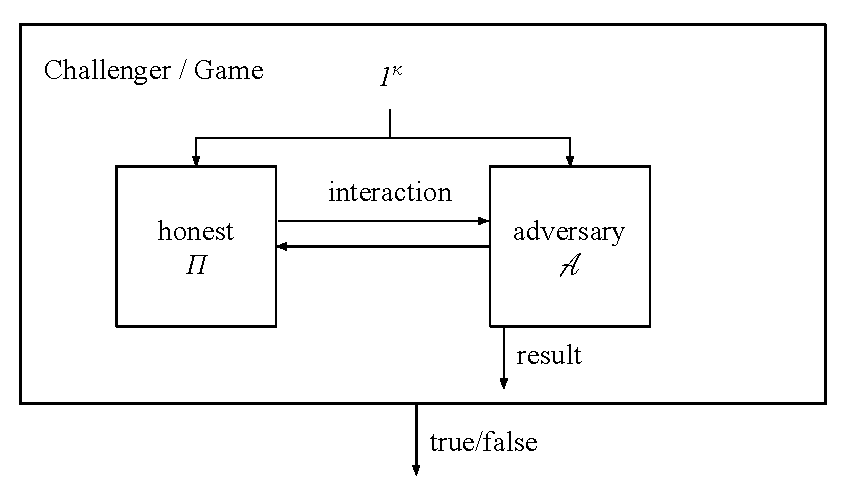
\includegraphics[width=0.7 \columnwidth,keepaspectratio]{figures/game-based-security.pdf}
    \caption{A game-based security definition shown diagramatically. The challenger invokes both
    the honest party and the adversary before deciding whether the adversary was successful.}
    \label{fig.game}
\end{figure}

\import{./}{algorithms/alg.game.tex}

\subsection*{Negligibility}

In an ideal world, we would like to state that our protocols are unbreakable:

\begin{quote}
  \textsf{my-game}$_{\Pi,\mathcal{A}}$($\kappa$) = \textsf{false}
\end{quote}

However, this goal is sadly unattainable. When the time comes to generate a secret
key or a password, we will make these have bit length $\kappa$. Unfortunately, the adversary
can \emph{guess} such secrets by taking a random guess. If our secret is sampled from the
set $\{0, 1\}^\kappa$, the set of $\kappa$-bit strings, the probability of the adversary
guessing correctly will be $2^{-\kappa}$. This is a probability of failure that we are
willing to accept, as it is unavoidable.

What happens if an adversary attempts to perform multiple guesses for the secret key?
Each of these guesses has a probability of success amounting to $\frac{1}{2^\kappa}$.
Since the adversary has polynomial time $p(\kappa)$, the number of guesses she can
perform must be polynomial, too. What is the probability that \emph{at least one of
these guesses} is correct? We can apply a \emph{union bound}~\cite{ross} to find this.

\begin{theorem}[Union Bound]
  Consider $n$ events $X_1, X_2, \cdots, X_n$. Then the probability
  that \emph{any one of them} occurs is given by their \emph{union bound}:

  \[
    \Pr[X_1 \lor X_2 \lor \cdots \lor X_n] \leq \Pr[X_1] + \Pr[X_2] + \cdots + \Pr[X_n]
  \]
\end{theorem}

Note that this is just an upper bound and these probabilities may not be exactly
equal. To see why, consider the simple example of rolling a die $6$ times, hoping
to get a $6$. For any one roll, the probability of getting a $6$ is $\frac{1}{6}$,
and the union bound tells us that the probability of getting a $6$ in \emph{any
roll} across our whole game of $6$ rolls is at most $1$. However, the actual probability
is in fact a little less: $1 - (1 - \frac{1}{6})^6 = 0.665$. Here, we calculated
the probability of \emph{not} winning in a single roll, which is $1 - \frac{1}{6}$.
We then calculated the probability of failing to win in any single roll, which is
$(1 - \frac{1}{6})^6$. Lastly, we took the complement of this probability, interpreting
this to mean that we won in at least a single roll, obtaining $1 - (1 - \frac{1}{6})^6$.
We will use this style of arguments a lot when counting probabilities about blocks
and chains.

Returning to our polynomial adversary, and applying a union bound, we see that
this adversary can succeed with probability bounded by $\frac{p(\kappa)}{2^\kappa}$.

If we have one adversary who can succeed with some probability $Pr_\mathcal{A}$,
then a different adversary $\mathcal{A}'$ can succeed with probability
bounded by $p(\kappa) Pr_{\mathcal{A}}$ for any polynomial $p$. This is known as
\emph{amplification}\index{Amplification}.
We wish to define a class of probability functions that we deem \emph{acceptable}
probabilities of failure. Clearly, if an adversary has a \emph{constant} probability of success
(such as $0.5$) that does not depend on the security parameter $\kappa$, this is \emph{not}
acceptable, as we want $\kappa$ to be our \emph{tuning knob} of how secure our protocol will be.
We will deem \emph{acceptable} the class of functions denoting a probability which is not
amplifiable to a constant by this manner.

Any inverse polynomial probability such as $\frac{1}{\kappa^3 + \kappa + 9}$ can be amplified by a
polynomial adversary to be close to the union bound by repeating the experiment a polynomial
number of times. Therefore, we must ask that our probability is \emph{smaller than any inverse
polynomial}. Such functions are called \emph{negligible}.

\begin{definition}[Negligible function]\index{Negligible function}
  A function $f(\kappa)$ is \emph{negligible} if for any polynomial degree
  $m \in \mathbb{N}$, there exists a $\kappa_0$ such that for all
  $\kappa > \kappa_0$:

  \[
    f(\kappa) < \frac{1}{\kappa^m}
  \]
\end{definition}

We choose to accept negligible functions exactly because the probability of failure
cannot be amplified in this manner. If an adverary $\mathcal{A}$ succeeds with negligible
probability, an adversary $\mathcal{A}'$ that simulates $\mathcal{A}$ must run the
simulation an \emph{exponential} number of times in order to achieve anything beyond
a negligible probability. Given that we have constrained our adversaries to be polynomial-time,
this is impossible.

The negligible probability of failure is the standard treatment in modern cryptography~\cite{katz}.
Beyond the above argument pertaining to the polynomiality of adversaries, negligible
functions are easy to work with because they observe certain \emph{closure} properties.
In particular, multiplying a negligible function with a polynomial yields a negligible
function. As constants are polynomials, scaling a negligible function by a constant
yields a negligible function too. Of course, multiplying something negligible with
something negligible keeps it negligible, and taking any constant power of a negligible function
keeps it negligible.

\begin{align*}
  \textsf{negl} \cdot \textsf{negl} &= \textsf{negl}\\
  \textsf{const} \cdot \textsf{negl} &= \textsf{negl}\\
  \textsf{poly} \cdot \textsf{negl} &= \textsf{negl}\\
  \forall k \in \mathbb{N}: \textsf{negl}^k &= \textsf{negl}
\end{align*}

\subsection*{Definitions of Security}

As designers, the ideal goal for us would be to design a protocol for which \emph{no adversary}
succeeds in breaking the game, no matter what code she is running. If we can achieve this, it
will be a truly magnificent achievement. Observe what we are trying to say here: The protocol
works \emph{no matter what the adversary decides to do}, as long as our assumptions are respected
(such as the polynomiality bounds on the adversary).
We are not merely enumerating a bunch of attacks that we considered ourselves and arguing that
our protocol is secure against \emph{these}!
Instead, we are arguing against \emph{all adversaries}, even adversaries that we do
not know about and have not imagined. The ability to argue against \emph{all} adversaries is the
epitome of modern cryptography, a feat only possible through the
formalism and models of computer science. This proof style is recent and has only appeared within
the last 50 years.

The ideal protocol $\Pi$ satisfies security against all adversaries:

\[
  \forall PPT \mathcal{A}: \textsf{Game}_{\Pi,\mathcal{A}}(\kappa) = 0
\]

However, this is an unattainable goal. To see this, consider the case where the honest party
generates a secret of length $\kappa$ such as a private key or password. In that case the
adversary can simply attempt to \emph{guess} this private key at random. This will be possible
with probability $\frac{1}{2^\kappa}$. As such, the above goal of requiring that the game
\emph{always} outputs $0$ for all adversaries cannot be attained. Instead, we will require
that any adversary only has negligible probability of succeeding in breaking these games.
Remember that the probability of randomly finding the secret key is $\frac{1}{2^\kappa}$
and this is a negligible value in $\kappa$.

A security definition will look like this:

\begin{definition}[Security]
  A protocol $\Pi$ is secure with respect to game $\textsf{Game}$ if there exists a negligible
  function $\textsf{negl}(\kappa)$ such that

  \[
    \forall PPT \mathcal{A}: \Pr[\textsf{Game}_{\Pi,\mathcal{A}}(\kappa) = 1] \leq \textsf{negl}(\kappa)
  \]
\end{definition}

We are using probability notation here because the execution of the challenger \emph{with the
same honest protocol $\Pi$ and against the same adversary $\mathcal{A}$ and using a fixed security parameter
$\kappa$} will not always yield
the same result! Since both the honest party and the adversary have access to generate randomness,
the challenger will sometimes report $0$, and other times report $1$. For a fixed $\Pi$ and $\mathcal{A}$
and $\kappa$, there is a certain probability that the challenger will report $0$, and a certain
probability that the challenger will report $1$.

Fixing $\Pi$ and $\mathcal{A}$, but leaving $\kappa$
to take any value, we obtain different probabilities for each value of $\kappa$. Therefore,
the value denoted by $\Pr[\textsf{Game}_{\Pi,\mathcal{A}}(\kappa) = 0]$ for a fixed $\Pi$ and
$\mathcal{A}$ is a function of $\kappa$. What we are saying here is that this function that
counts the probability must be below some negligible function. Said differently, that probability
must \emph{eventually} (for sufficiently large $\kappa$) become smaller than all inverse polynomials.

\subsection*{The Honest/Adversarial Gap}

Note here how great the requirements of security that cryptography mandates are:
In a \emph{secure} protocol, the honest party can act within polynomial time,
but an adversary needs superpolynomial time to break it. The successful honest party
is efficient and lives within the
complexity class \textsc{P}, but the successful adversary is inefficient, and
lives within the complexity class \textsc{NP} but not in \textsc{P}. This is
illustrated in Figure~\ref{fig.p-vs-np}. This is a much bolder claim that the
security of traditional money! In a traditional banknote monetary system, the honest party
(such as the government) has many more resources than the adversary (say, a forgery
criminal). If the adversary acquires resources equivalent to the honest party (for example
access to the same banknote-printing machines), the system's security will be
compromised. Here, we are achieving something significantly stronger: An honest
party needs only polynomial time to successfully participate in the protocol,
but a successful adversary will require superpolynomial time to successfully break it
--- a huge discrepancy.

\begin{figure}[h]
    \centering
    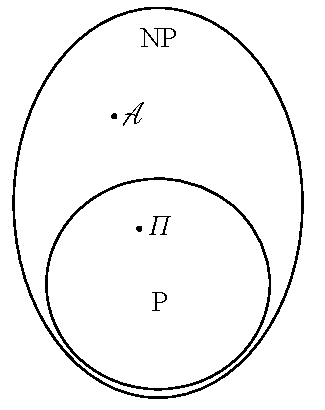
\includegraphics[width=0.3 \columnwidth,keepaspectratio]{figures/p-vs-np.pdf}
    \caption{In a secure protocol, a successful honest party needs polynomial time,
    while a successful adversary needs superpolynomial time.}
    \label{fig.p-vs-np}
\end{figure}

\subsection*{Proofs of Security}

When the time comes to prove a protocol secure, we will sometimes make an assumption
that an existing, underlying protocol is secure. Our new protocol will be built
\emph{on top of} the existing protocol. In the blockchain world, we will take many
underlying primitives for granted: We will make use of \emph{hash functions}
and \emph{signatures} assuming they are secure, and leave their design to the
cryptographers. Our theorems will state that \emph{if} the underlying protocol is
secure, \emph{then} the protocol we are building on top of the existing primitive
is also secure. Said differently, if no PPT adversary wins in the underlying protocol
except with negligible probability, then also no PPT adversary can win in our new
protocol, except with negligible probability.

The proofs of these theorems will take the form of a \emph{computational reduction},
and they will look roughly as follows, when we are designing a new protocol $\Pi^*$:

\noindent
\textbf{Claim. } If protocol $\Pi^*$ is secure, then protocol $\Pi$, built on top of $\Pi^*$,
is also secure.

\noindent
\textbf{Proof. } Suppose, towards a contradiction, that protocol $\Pi$ is \emph{insecure}.
Then, by the game-based security definition, there must exist a PPT adversary $\mathcal{A}$
that breaks $\Pi$ with non-negligible probability (but we don't know the exact inner workings
of this adversary, because she is arbitrary).
We design a PPT adversary $\mathcal{A}^*$, for which we write the code
and know her inner workings \emph{exactly}. Somewhere in the code of $\mathcal{A}^*$ we make
use of the code of $\mathcal{A}$ as a black box. The adversary $\mathcal{A}^*$ attempts
to break the protocol $\Pi^*$ within the confines of the challenger for the protocol $\Pi^*$
(a particular game).
The adversary $\mathcal{A}$ attempts to break the protocol $\Pi$ within the confines of
the challenger for the protocol $\Pi$ (a different game).
When $\mathcal{A}^*$ runs, she \emph{simulates}
the execution of $\mathcal{A}$ by invoking her code, as illustrated in
Figure~\ref{fig.reduction}. When $\mathcal{A}^*$ invokes
$\mathcal{A}$, she must do so behaving \emph{as if she were} the challenger for protocol
$\Pi$. The adversary $\mathcal{A}^*$ can invoke $\mathcal{A}$ multiple times with
different inputs and collect her outputs before producing an output of her own.
Because $\mathcal{A}$ runs in polynomial time, and because $\mathcal{A}^*$ only
performs a polynomial number of operations beyond invoking $\mathcal{A}$ a polynomial
number of times, therefore $\mathcal{A}^*$ is also a PPT. We can now evaluate the
probability of success of $\mathcal{A}^*$ and relate it to the probability of success
of $\mathcal{A}$, arguing that \emph{if} the probability of success of $\mathcal{A}$
is non-negligible, then so is the probability of success of $\mathcal{A}^*$. However,
this contradicts the assumption that $\Pi^*$ was secure, completing the proof. $\lozenge$

\begin{figure}[h]
    \centering
    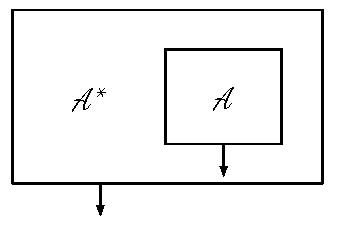
\includegraphics[width=0.4 \columnwidth,keepaspectratio]{figures/reduction.pdf}
    \caption{A computational reduction between two adversaries. Given an adversary
    $\mathcal{A}$ against protocol $\Pi$, we construct an adversary $\mathcal{A}^*$
    against a protocol $\Pi^*$.}
    \label{fig.reduction}
\end{figure}

This proof style is by contradiction. We can write the same proof in a \emph{forward
direction} without resorting to a contradiction. This gives a shorter proof, and we
will prefer this style in our writing, following the example of Katz and
Lindell~\cite{katz}. These proofs look like this:

\noindent
\textbf{Proof. } Consider an arbitrary PPT adversary $\mathcal{A}$ attempting to break
the protocol $\Pi$. We construct an adversary $\mathcal{A}^*$ against the protocol
$\Pi^*$ by making use of $\mathcal{A}$ as before. For the same reasons as before,
$\mathcal{A}^*$ is also PPT, and their probabilities of success are related. By the
security assumption on $\Pi^*$, we know that the probability of success of $\mathcal{A}^*$
against its challenger is negligible. From the relationship between the probabilities
of success of $\mathcal{A}$ and $\mathcal{A}^*$, we also deduce that the probability
of success of $\mathcal{A}$ is negligible, completing the proof. $\lozenge$

The two proofs are identical, with the exception that the second one is a little more
straightforward. Of course, these are rough proof outlines provided to give a sketch
of what to expect next, but are still quite abstract.
You will become acquainted with the particular workings of this style of proof as we work
through particular theorems, particular protocols, and particular games in the next chapters.

\section{The Network}

In our quest to decentralize money, our participants will be nodes on a computer network.
These nodes will each run their software and communicate with one another. Each of them
is connected to some of their \emph{peers} as illustrated in Figure~\ref{fig.network}.
Contrary to more traditional Internet systems where there is a designated role of a
\emph{client} and a \emph{server}, here all peers play the same role: They function both
as clients and as servers of requests.

\begin{figure}[h]
    \centering
    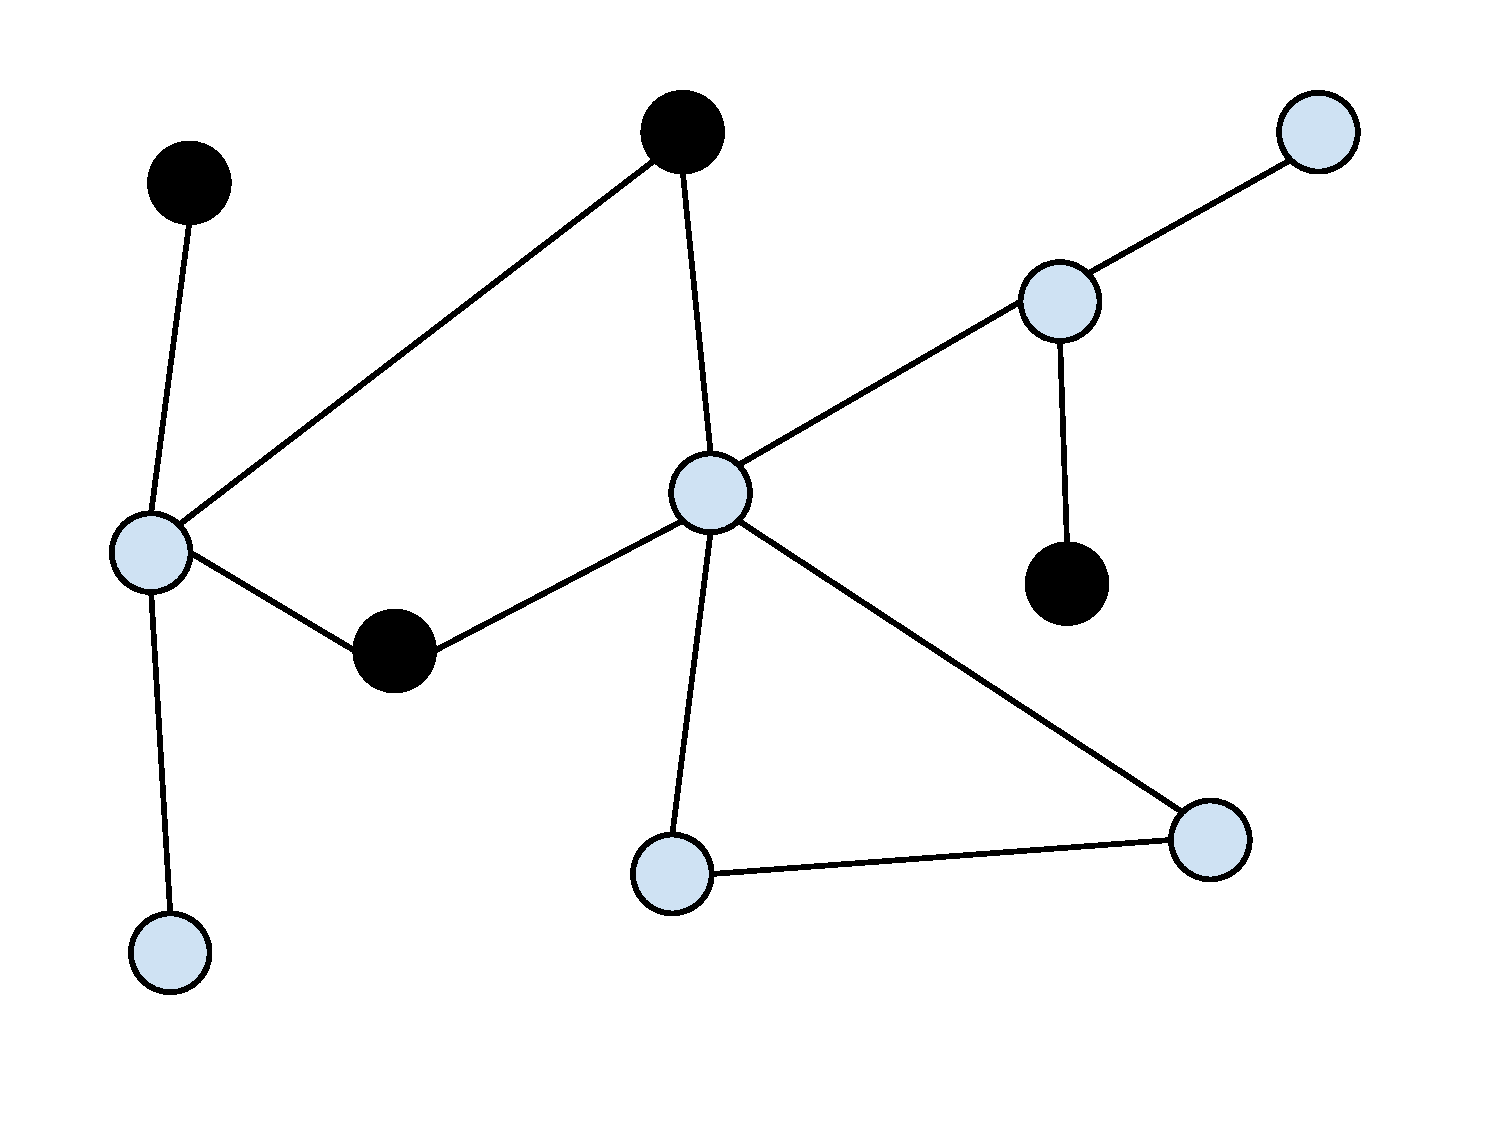
\includegraphics[width=0.5 \columnwidth,keepaspectratio]{figures/peer-to-peer-network.pdf}
    \label{fig.network}
    \caption{The peer-to-peer network. Nodes are shown as circles and connections as lines.
    The honest nodes are shown in blue, while the adversarial nodes are shown in black.}
\end{figure}

\subsection*{The Non-Eclipsing Assumption}

In this network, not everyone is connected to everyone else, but messages can reach from
one side of the network to the other by travelling through intermediaries. This is achieved
through the \emph{gossiping}\index{Gossip} protocol: When a node receives a message it hasn't seen before,
it forwards it to its peers. That way, everyone eventually learns about the message. In order
to avoid denial-of-service attacks, messages may be validated in a basic manner before they
are gossiped. For example, syntactically invalid messages will not be gossiped.

We will make a central assumption about the network: That there exists a path between any two honest parties on the network, which consists of only honest nodes. Said differently, the network is not split into components whose connection is controlled by the adversary.

\begin{definition}[Non-eclipsing]
  The \emph{non-eclipsing assumption} states that,
  between every two honest parties on the network, there exists a path consisting only of honest nodes.
\end{definition}

Note that, for the non-eclipsing assumption to hold, it is \emph{not} sufficient that every honest party
has a connection to an honest party. There might be components of honest parties that remain
isolated from the rest of the network, as illustrated in Figure~\ref{fig.eclipsing}.

\begin{figure}[h]
    \centering
    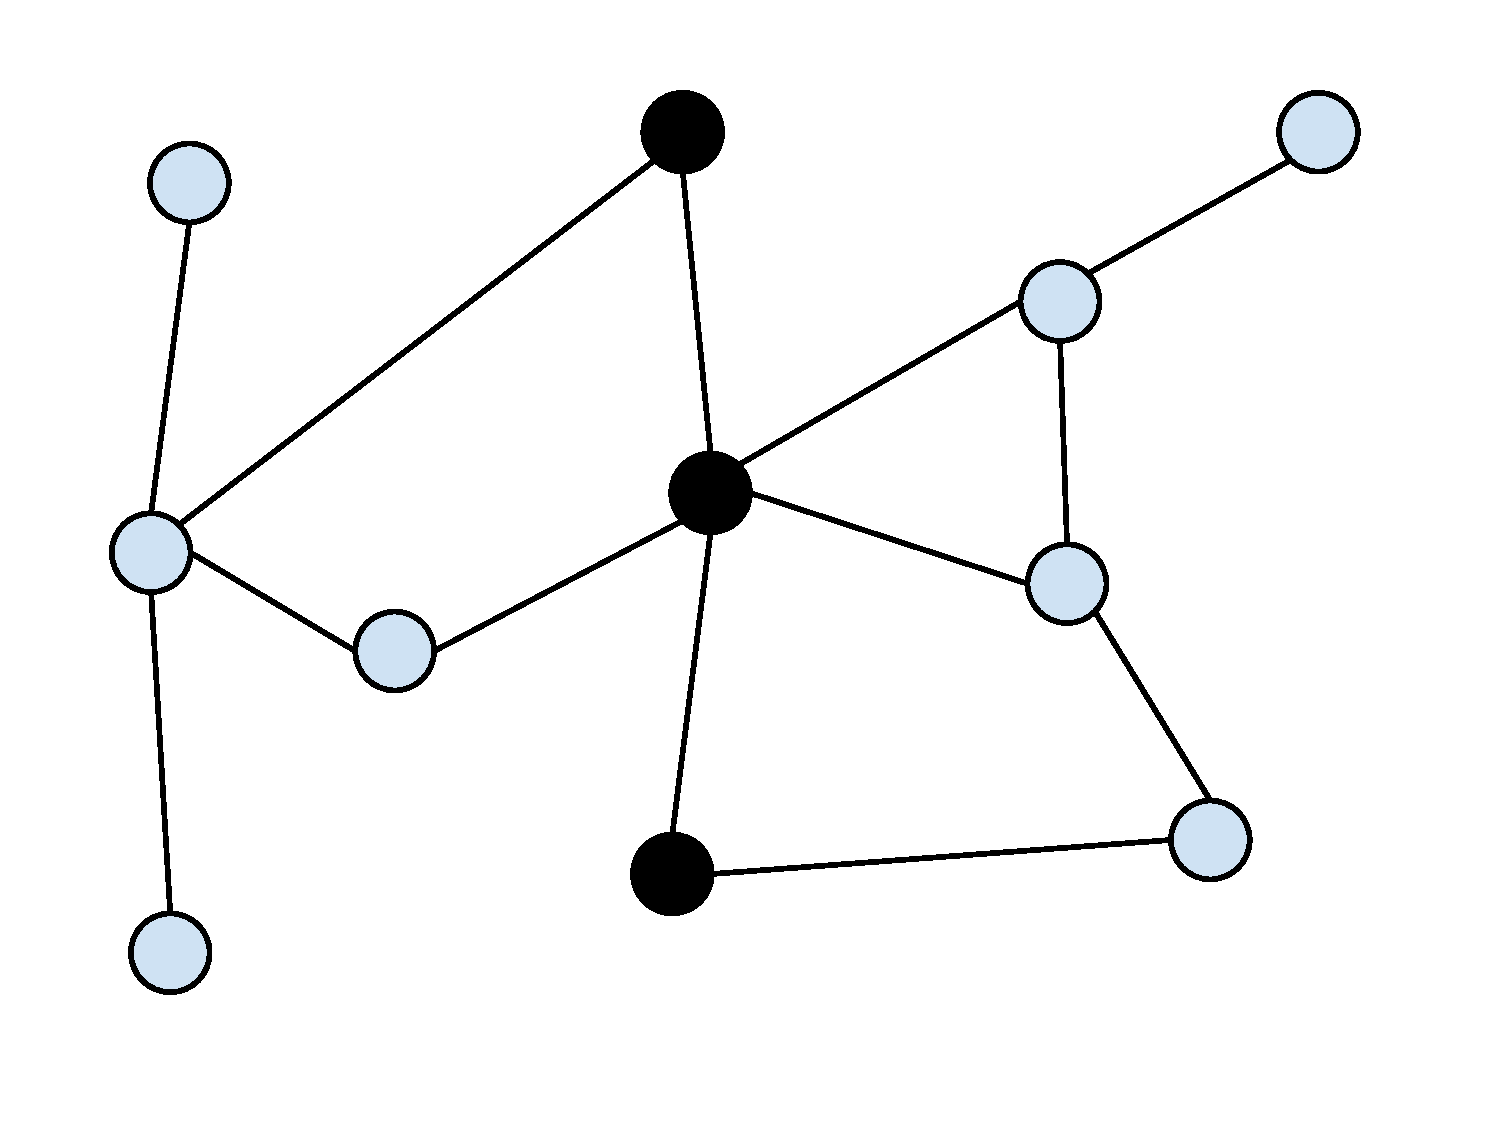
\includegraphics[width=0.5 \columnwidth,keepaspectratio]{figures/eclipsed-peer-to-peer-network.pdf}
    \caption{An eclipsed peer-to-peer network. Even though every honest party has an honest connection,
    the network is partitioned into two disconnected components by the adversary.}
    \label{fig.eclipsing}
\end{figure}

We are introducing this assumption out of necessity. We cannot hope to build any currency
in an eclipsed world. To see why, imagine two completely isolated civilizations, both maintaining
their own separate currency. These civilizations, given a lack of communication between them, cannot
hope to be able to deduce who owns how much money in their respective counterpart world.

\subsection*{The Sybil Attack}

\begin{figure}[h]
    \centering
    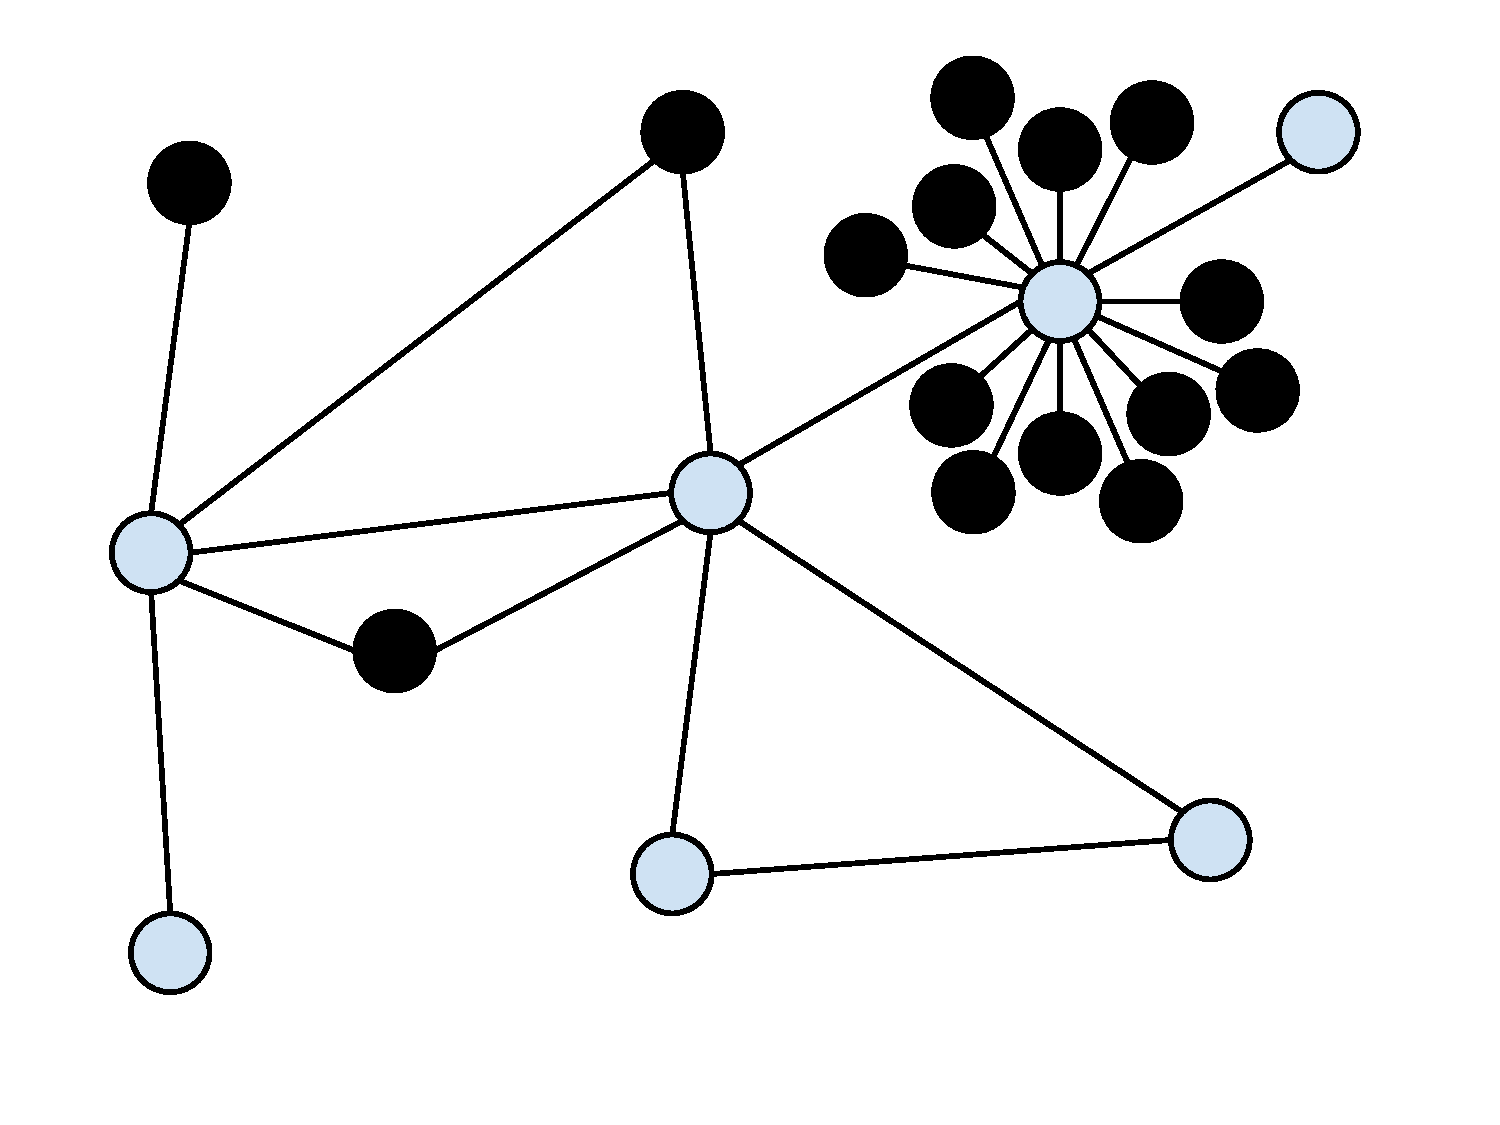
\includegraphics[width=0.5 \columnwidth,keepaspectratio]{figures/sybil-attack.pdf}
    \caption{A Sybil attacked peer-to-peer network. The non-eclipsing assumption is not violated.}
    \label{fig.sybil}
\end{figure}

Following our pattern of a powerful adversary, we give the adversary the ability to create
as many identities on the network as she desires. This is termed a
\emph{Sybil attack}~\cite{sybil}\index{Sybil Attack}. The adversary may overwhelm an honest party with adversarial
connections as illustrated in Figure~\ref{fig.sybil}.

\begin{definition}[Sybil Attack]
  In a \emph{Sybil attackable} network model, the adversary may create as many identities (nodes)
  as she desires. The honest parties cannot distinguish which identities have been created by
  the adversary in this manner.
\end{definition}

It is possible that the adversary controls all the connections of an honest party, except for
one connection to an honest party, which is necessary to maintain the non-eclipsing assumption.
\emph{Every honest party will certainly be connected to at least one other honest party.}

\subsection*{Peer Discovery}

Ensuring that the non-eclipsing assumption is maintained is a practical engineering problem and
there are many heuristics employed in achieving this. The process of connecting to other nodes,
attempting to ensure at least one honest connection, is termed \emph{peer discovery}\index{Peer Discovery}.

Let us briefly discuss how peer discovery is performed in practical peer-to-peer
networks. When a peer-to-peer node is first booted, it must connect to some of its peers for the
first time. This is the \emph{network bootstrapping}\index{Bootstrapping} phase. At this phase, the node typically
will attempt to connect to a list of hard-coded peers whose IP addresses appear in the implementation
source code. Some of these connections may fail, but if one of them succeeds and connects to an honest
party, the newly booted node can begin to operate. After bootstrapping, whenever the newly booted node connects
to a peer, it asks the connected peer to tell it about the addresses of \emph{its own peers}. These
peers are then recorded and can be used for further connections. They can also be reported to other
peers asking for peer discovery. The policy for reporting discovered peers may vary. For example,
some nodes may not share all of their known peers. In case the bootstrapping phase fails, the user
is given the option to manually connect to a peer by entering its address. This allows the software
to survive cases of censorship, or of broad compromise of all the hard-coded peer addresses.

\section*{Problems}

\begin{enumerate}
  \item Which of the following functions are negligible in $\kappa$?
    \begin{enumerate}
      \item $f(\kappa) = 0$
      \item $f(\kappa) = 1$
      \item $f(\kappa) = 2^{-128}$
      \item $f(\kappa) = \frac{2^\kappa}{128}$
      \item $f(\kappa) = \frac{128}{2^\kappa}$
      \item $f(\kappa) = \frac{1}{3\kappa^3 + 7\kappa^2 + 12}$
      \item $f(\kappa) = \frac{\kappa^{7}}{7^{\kappa}}$
      \item $f(\kappa) = \frac{1}{\log \kappa}$
      \item $f(\kappa) = \frac{1}{\kappa!}$
    \end{enumerate}
  \item Use induction to prove the \emph{Union Bound} theorem.
  \item Let $f$ and $g$ be negligible functions. Show that $h(\kappa) = \max\{f(\kappa), g(\kappa)\}$
        is negligible.
  \item Prove that
    \begin{enumerate}
      \item $\textsf{negl} \cdot \textsf{negl} = \textsf{negl}$
      \item $\textsf{const} \cdot \textsf{negl} = \textsf{negl}$
      \item $\textsf{poly} \cdot \textsf{negl} = \textsf{negl}$
      \item $\forall m \in \mathbb{N}: \textsf{negl}^m = \textsf{negl}$
    \end{enumerate}
\end{enumerate}

\section*{Further Reading}

Blockchain science is founded on cryptography. For a great introduction to modern cryptography,
consult \emph{Introduction to Modern Cryptography} by Katz and Lindell~\cite{katz}. It is a beautifully
written book. It explores how to build many of the primitives we will make use throughout this book,
including hash functions and signature schemes. More importantly, it is a good way to learn about the
adversarial mindset and to look into complexity reduction-based security proofs. The book is filled with
theorems and proofs that show that, for all PPT adversaries, the protocol is secure, except with negligible
probability. In \emph{Further Reading} paragraphs at the end of the next chapters, you will find
some references in chapters of \emph{Modern Cryptography} (2nd edition).
Another good book on cryptography is \emph{Foundations of Cryptography}~\cite{foundations1,foundations2}.
An easier and pleasant to read textbook is Smart's \emph{Cryptography Made Simple}~\cite{smart}.

For a more in-depth treatment of Turing Machines and our computational model, consult Sipser's
\emph{Introduction to the Theory of Computation}~\cite{sipser}. It is a very well written book,
with great examples and proofs that are written to be educational. It's an easier book than
\emph{Modern Cryptography}, and a good way to learn computational reductions.

Throughout this book, we use many elements of discrete mathematics and probability theory. For
discrete mathematics, you can use Liu's \emph{Elements of Discrete Mathematics}~\cite{liu}.
For probability theory, you can use Ross's
\emph{A First Course on Probability Theory}~\cite{ross}. You can read both cover-to-cover, but
they also function well as a reference in case you want to look something up.
